\subsection{BWV1}

O sexto movimento de \emph{Wie schün leucht der Morgenstern} (Cantata para a festa da Anunciação, 1725, ver figura \ref{fig:bwv_frag})\footnote{Vídeo disponível em \url{https://www.youtube.com/watch?v=POe2fBjbswA}.} foi utilizado segundo procedimentos explicados na seção \ref{sec:metodo}. Foi gerado um conjunto de simultanóides\footnote{Utilizo aqui a nomenclatura de \cite{koellreutter_introducao_1987} para identificar blocos harmônicos.}, apresentado na figura \ref{fig:bwv1_extract}.

\begin{figure}[h]
  \centering
  {%
\parindent 0pt
\noindent
\ifx\preLilyPondExample \undefined
\else
  \expandafter\preLilyPondExample
\fi
\def\lilypondbook{}%

\includegraphics{../examples/bwv1/c7/lily-6fc7e149-1}%
\ifx\betweenLilyPondSystem \undefined
  \linebreak
\else
  \expandafter\betweenLilyPondSystem{1}%
\fi

\includegraphics{../examples/bwv1/c7/lily-6fc7e149-2}%
\ifx\betweenLilyPondSystem \undefined
  \linebreak
\else
  \expandafter\betweenLilyPondSystem{2}%
\fi

\includegraphics{../examples/bwv1/c7/lily-6fc7e149-3}%
% eof

\ifx\postLilyPondExample \undefined
\else
  \expandafter\postLilyPondExample
\fi
}

  \caption{Sequência de simultanóides gerados. \textbf{Fonte}: Autor.}
  \label{fig:bwv1_extract}
\end{figure}

 Cada bloco harmônico são notas de um determinado compasso, escolhido ao acaso pelo programa, comprimidas em um único evento. Algumas notas podem ter sido omitidas por erros de codificação no \emph{script} Python. Mas isso é coerente com o princípio estético. É também  interessante observar uma direcionalidade da tessitura, que vai da região média aos graves, percebida após repetidos usos do comando descrito. 

Realizei algumas intervenções com este material: \begin{itemize}
\item manutenção da ordem dos blocos;
\item escolha de pontos que delimitam fraseados (silêncio como articulado de frases;);
\item observação de densidades na quantidade de notas como fator para o fim do fraseado;
\item dinâmicas como um dispositivo de ênfase do fraseado harmônico; 
\item a modificação de uma oitava de dois si bemoís para um intervalo de sétima ou nona de si bequadro e si bemol compasso, inserindo um intervalo de sétima com outro sib;  
\item deslocamento ou subtração de elementos da figura \ref{fig:bwv1_extract}.
\end{itemize}

A peça finalizada está na figura \ref{fig:bwv1}.

 \begin{figure}
  \centering
  {%
\parindent 0pt
\noindent
\ifx\preLilyPondExample \undefined
\else
  \expandafter\preLilyPondExample
\fi
\def\lilypondbook{}%

\includegraphics{../examples/bwv1/d8/lily-ef199858-1}%
\ifx\betweenLilyPondSystem \undefined
  \linebreak
\else
  \expandafter\betweenLilyPondSystem{1}%
\fi

\includegraphics{../examples/bwv1/d8/lily-ef199858-2}%
\ifx\betweenLilyPondSystem \undefined
  \linebreak
\else
  \expandafter\betweenLilyPondSystem{2}%
\fi

\includegraphics{../examples/bwv1/d8/lily-ef199858-3}%
\ifx\betweenLilyPondSystem \undefined
  \linebreak
\else
  \expandafter\betweenLilyPondSystem{3}%
\fi

\includegraphics{../examples/bwv1/d8/lily-ef199858-4}%
% eof

\ifx\postLilyPondExample \undefined
\else
  \expandafter\postLilyPondExample
\fi
}

  \caption{Peça resultante das intervenções. \textbf{Fonte}: autor.}
  \label{fig:bwv1}
\end{figure}

As ferramentas analíticas auxiliaram a observação de semelhanças e diferenças entre uma peça original  e a peça variada. Por exemplo, com BWV1 de J.S.Bach, o histograma da figura \ref{fig:pitch-class-bwv1-histogram} revela fatos analíticos comuns, como uma ênfase do \emph{pitch class} 5, Fá, I grau; e depois \emph{pitch class} 0, Dó, V grau, seguido de outras classes, como Lá (III grau) e Sol (ii grau ou V/V); outros, como Ré (vi grau) e Si bemol, possuem a mesma quantidade. Por último Mi (vii grau) e si natural possuem menor número, talvez como dispositivos cadenciais(como por exemplo na ``modulação'' Fá$\Rightarrow$Dó do quinto compasso da figura \ref{fig:bwv_frag}).

A partir da artesania do material pré-composicional gerado por fragmentação do BWV1, notei, no histograma da figura \ref{fig:pitch-class-bwv1-histogram-2} que algumas proporções foram mantidas de maneira aproximada. A quantidade de eventos diminui drasticamente. Mesmo com a segmentação da peça, um centro tonal ainda pode ser notado (embora de maneira bastante ambígua).

\begin{figure}[!h]
  \centering
  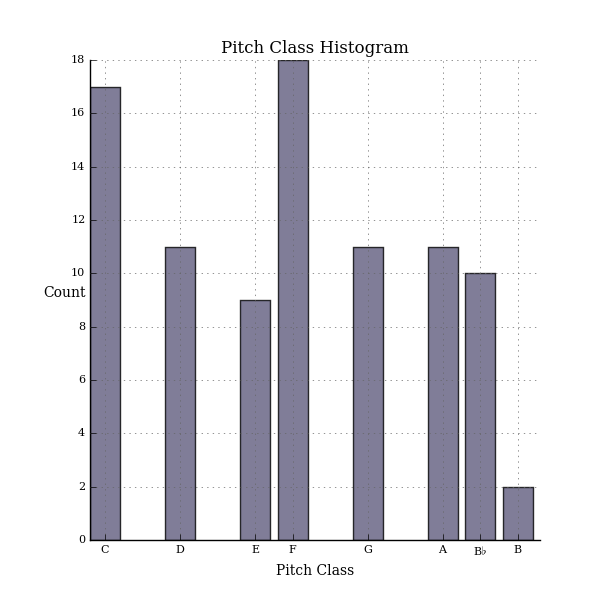
\includegraphics[scale=0.71]{../analysis/bwv1/pitch-class-1.png}
  \caption{Histograma de \emph{pitch-class} da peça feita, utilizando o comando \emph{./main.py -x examples/bwv1/bwv1.xml --plot-histogram-pitch-class}}
    \label{fig:pitch-class-bwv1-histogram-2}
\end{figure}

